% !TEX program = xelatex
\documentclass[12pt]{book}
\usepackage{etex}
\usepackage{ctex}
\usepackage{authblk}
\usepackage{amsmath}
\usepackage{graphicx}
\usepackage{subfig}
\usepackage{geometry}
\geometry{a4paper,scale=0.8}
\def\celsius{\ensuremath{^\circ\hspace{-0.09em}\mathrm{C}}}
\numberwithin{equation}{section}
\usepackage{tabu}
\usepackage{booktabs}
\usepackage[numbers,sort&compress]{natbib}
\newcommand*{\dif}{\mathop{}\!\mathrm{d}}
\usepackage{caption}
\usepackage[section]{placeins}
\usepackage{float}
\usepackage{placeins}
\DeclareTextFontCommand{\emph}{\bfseries}
\usepackage{verbatim}
\usepackage{amsmath,amssymb}
\usepackage{inputenc}
\usepackage{xeboiboites}
\usepackage{verbatim}
\usepackage{amsmath,amssymb}
\usepackage{braket}
\usepackage{siunitx}
\usepackage{tikz}
\usetikzlibrary{intersections}
\usepackage{pgfplots}
\pgfplotsset{compat=1.16,width=7cm}
\usepackage{makeidx}
\usepackage[version=4]{mhchem}
\makeindex
%\usepackage{microtype}

%\usepackage{lipsum}
%opening
\title{固体物理}
\author{Kars}
\date{\today}

\DeclareTextFontCommand{\emph}{\bfseries}


\newboxedtheorem[
small box style={fill=gray!20,draw=black, rounded corners},
big box style={fill=gray!10,draw=orange,thick,rounded corners},
headfont=\bfseries,
thcounter=section]{define*}{Definition}{}

\newboxedtheorem[
small box style={fill=gray!20,draw=black, rounded corners},
big box style={fill=gray!10,draw=orange,thick,rounded corners},
headfont=\bfseries,
thcounter=subsection]{define}{Definition}{definecounter}

\newbreakabletheorem[small box style={draw=orange,fill=blue!20},
big box style={fill=blue!10,draw=orange}]
{theorem}{Theorem}{theoremcounter}
\newbreakabletheorem[small box style={draw=orange,fill=blue!20},
big box style={fill=blue!30,draw=orange}]
{theorem*}{Theorem}{}
\newbreakabletheorem[small box style={fill=white!20,draw=black, 
	rounded corners},
big box style={fill=white!10,draw=orange,thick,rounded corners},
headfont=\bfseries,
broken edges={draw=orange!30!black!20,thick,fill=orange!20!black!5, 
	decoration={random steps, segment length=.5cm,%
		amplitude=1.3mm},decorate},%
other edges={decoration=penciline,decorate,thick}]%
{example}{Example}{examplecounter}    
\newboxedtheorem[small box style={fill=blue!20,draw=black, 
	rounded corners},
big box style={fill=blue!10,draw=orange,thick,rounded corners},
headfont=\bfseries]%
{example*}{Example}{}  

\newboxedtheorem[small box style={fill=blue!10,draw=black, line width=.7pt,
	decoration={penciline},decorate},%
big box style={fill=blue!10,draw=black,thick, 
	decoration={penciline},decorate},
headfont=\bfseries]%
{Proof}{Proof}{}


\newboxedequation[big box style={fill=blue!10,%
	thick,decoration=penciline,decorate}]%
{formula}      



\newbreakabletheorem[small box style={draw=orange,fill=blue!20},
big box style={fill=blue!10,draw=orange},
broken edges={decoration=zigzag}]
{propd}{Proposition}{test}    

\newbreakabletheorem[small box style={draw=orange!30!black!20,%
	fill=orange!10!black!2,decoration=penciline, decorate, thick},
big box style={color=orange!30!black!20,fill=orange!30!black!10,thick},
broken edges={draw=orange!30!black!20,thick,fill=orange!20!black!5, 
	decoration={random steps, segment length=.5cm,%
		amplitude=1.3mm},decorate},%
other edges={decoration=penciline,decorate,thick}]%
{parchment}{Parchment}{test}    

\newparchment[small box style={draw=orange!30!black!20,%
	fill=orange!10!black!2,decoration=penciline, decorate, thick},
big box style={color=orange!30!black!20,fill=orange!30!black!10,thick},
broken edges={draw=orange!30!black!20,thick,fill=orange!20!black!5, 
	decoration={random steps, segment length=.4cm,%
		amplitude=1.7mm},decorate},%
other edges={decoration=penciline,decorate,thick}]%
{parchmentb}{Parchment}{}     

\newspanning[image=dessins/bulb,headfont=\bfseries,%
spanning style={very thick,decoration=penciline,decorate}]%
{method}{Method}{}

\newspanning[image=dessins/poisson,headfont=\itshape,%
spanning style={very thick,decoration=penciline,decorate}]%
{test}{Test}{}
\usepackage{hyperref}
\hypersetup{
	colorlinks,
	citecolor=black,
	filecolor=black,
	linkcolor=black,
	urlcolor=black
}
\usepackage{cleveref}
\begin{document}

\maketitle



\tableofcontents
\clearpage
\section[Preface]{前言}
	笔记内容来自阎守胜先生的《固体物理基础》和黄昆先生的《固体物理学》以及课堂笔记。由于鄙人能力不足,
	课堂笔记部分和非常浅薄,因此主要使用阎先生的部分。
\part{理想晶体}
\chapter{能带理论}
\begin{define}
    电子的能带指\textbf{晶体}电子的能级,能带理论的主要任务就是去确定固体电子的能级。
\end{define}
作用:
\begin{itemize}
    \item 阐明固体的基本性质,比如振动谱,磁有序,电导率,热导率,光学介电函数。
    \item 预测新材料,解释新现象。
\end{itemize}
能带图:横坐标为波矢(量子数),纵坐标为能量。

能带和能带之间的间隙如何产生?

本课程所作的简化:
\begin{itemize}
    \item 绝热近似:多粒子变为多电子,认为原子核处于静止状态。
    \item 单电子近似,假设所有电子的哈密顿量为:
    \begin{equation}
        H_e=\sum_{i=1}\left[-\frac{1}{2}v_e(r_i)+\sum_{R_n}\frac{1}{4\pi\varepsilon_0}\frac{e^2}{|r_i-R_n|}\right]
    \end{equation}
    多电子变为单电子问题,但是当相互作用势不能忽略时,不能用单电子近似,比如超导现象。
    \item  周期场近似,假设所有晶体的分布一致。忽略晶格振动和晶体缺陷
\end{itemize}

\section{一维周期势场的电子运动}
\subsection{电子运动的方程}
周期性势场:
\begin{equation}
    V(x)=V(x+ni).
\end{equation}
运动方程:薛定谔方程(一维)

此处使用微扰法,电子的能量和波函数分别近似到二级和一级。

假设微扰项为:
\begin{equation}
    \Delta V=V(x)-\bar{V}.
\end{equation}
\begin{itemize}
    \item 一级微扰方程
    \item 零级波函数
    \item 边界条件与波矢的取值
    \begin{equation}
        k=\frac{2\pi l}{aN'}, l=0,\pm 1,\pm 2\cdots .
    \end{equation}
    当$N'$原胞数足够大时,可视为准连续\footnote{布里渊区的宽度与$a$晶体结构有关。}。
\end{itemize}

\subsection[Bloch Theorem]{布洛赫定理}
    当势场具有周期性边界条件(晶格势场),波函数满足满足如下性质
    \begin{equation}
        \varphi(r+\vec{R}_n)=e^{i\vec{k}\cdot \vec{R}_n}\varphi(r).
    \end{equation}
    其中$\vec{k}$为一矢量,其表明平移晶格矢量$\vec{R}_n$时,波函数只增加相位因子$e^{i\vec{k}\cdot \vec{R}_n}$。

\subsection{微扰计算(近自由电子近似)}
\begin{itemize}
    \item 微扰计算公式
    \subitem 能量微扰项
    \subitem 波函数微扰项 
    \item 微扰矩阵元,得出选择定则:K态只能散射到相差一个倒格矢$k_n=n\frac{2\pi}{a}$的位置。
\end{itemize}
如果$K=n\frac{\pi}{a}$出现简并情况,非简并微扰法不再适用,应当使用简并微扰法。

当波矢$k=n\frac{\pi}{a}$,符合选择定则的两个态进行线性组合
\begin{equation}
    \Psi^{(0)}=A\Psi^{(0)}_k+B\Psi^{(0)}_{k'}.
\end{equation}

除此之外,波矢接近Bragg反射条件的两个态的能量非常接近。借助简并微扰的思想,我们将能量很接近的两个线性组合
使其同时满足选择定则和Bragg反射条件。所得能量为:
\begin{align}
    E=T_n(1+\Delta^2)\pm\sqrt{4T^2_n\Delta^2+|V_n|^2},
    T_n= \frac{\hbar^2}{2m}\left(n\frac{\pi}{a}\right)^2.\\
\end{align}
结果讨论:
\begin{itemize}
    \item 在$k=\pm n\frac{\pi}{a}$此时$\Delta$很小
\end{itemize}
\subsection{能带与禁带}
能量本征值$E_k$是波矢$k$的函数,在零级近似,既有电子模型下的能谱为抛物线关系:
\begin{equation*}
    E_k^{(0)}=\frac{\hbar^2k^2}{2m}.
\end{equation*}
计入周期场的微扰作用后,能量在k空间倒格矢的中点,即$k=n\frac{\pi}{a}$处断开,
电子能量不能取值,禁带宽度为$2|V_n|$。

\section{三维周期场中的电子运动}
\subsection{模型和微扰计算}
\subsubsection{运动方程}
电子受到粒子周期性势场的作用,势场的起伏较小, 零级近似,用势场的平均值代替离子产生的势场
\begin{align}
    \text{势场的平均值},&\bar{V}=\frac{1}{\Omega}\int_{\Omega}V(\vec{r})\dif \vec{r},\\
    \text{周期性势场起伏量},&V(\vec{r})-\bar{V}=\Delta V.
\end{align}

\subsection{布里渊区和能带}

\subsection{紧束缚近似}
两原子接近时,核与电子之间的库仑力使电子能级分立,然后形成能带。晶体内不同量子数的原子处于不同的能带
能带的宽度与近邻原子的重叠电子云的交互作用成正比。
\chapter{金属自由电子气体模型}\label{chapter:金属自由电子气体模型}
\section{模型和基态性质}\label{section:模型和基态性质}
     {自由电子气体模型}的基本假定:
    \begin{itemize}
        \item[1] 忽略电子和离子实自间的相互作用,电子的自由运动范围仅在样品内部,离子实为保持体系电中性的均匀正电荷,类似于 {凝胶}。
        \item[2] 忽略电子与电子之间的相互作用,也就是 {独立电子近似}。
    \end{itemize}
    \subsection{单电子本征态和本征能量}\label{subsection:单电子本征态和本征能量}
        对于温度$T=0$,体积$V=L^3$内的$N$个自由电子,其中$L$为立方边的边长,独立电子近似使$N$个电子的问题转化为单电子问题。单电子的状态波函数
        为$\varphi(r)$描述,$\varphi(r)$满足的不含时的薛定谔方程为:
        \begin{equation}
            \left[-\frac{\hbar^2}{2m}\nabla^2+V(r)\right]\varphi(r)=\varepsilon(r)\label{不含时单电子薛定谔方程}.
        \end{equation}
        其中$V(r)$为电子在金属中的势能,$\varepsilon$为电子的本征能量,忽略电子离子实的相互作用,在凝胶体系内$V(r)$为常数势,
        可以简单取零,\autoref{不含时单电子薛定谔方程}可以写为:
        \begin{equation}
            -\frac{\hbar^2}{2m}\nabla^2\varphi(r)=\varepsilon\varphi(r).
        \end{equation}
        与电子在自由空间运动的情形相同,方程有平面波解,
        \begin{equation}
            \varphi(r)=Ce^{ik\cdot r}\label{未归一化单电子波函数},
        \end{equation}
        其中$C$为归一化常数,使得整个空间内的电子出现的概率为1
        \begin{equation}
            \int_V\left|\varphi(r)\right|^2\dif r=1.
        \end{equation}
        因此波函数\autoref{未归一化单电子波函数}也就可以写作
        \begin{equation}
            \varphi_k(r)=\frac{1}{\sqrt{V}}e^{ik\cdot r}\label{归一化单电子波函数},
        \end{equation}
        其中用以标记波函数的$k$是平面波的波矢,$k$的方向为平面波的传播方向,$k$的大小与波长$\lambda$的关系为
        \begin{equation}
            k=\frac{2\pi}{\lambda}\label{电子波矢与波长的关系}.
        \end{equation}
        将\autoref{归一化单电子波函数}代入\autoref{不含时单电子薛定谔方程}可得相应的电子能量为
        \begin{equation}
            \varepsilon(k)=\frac{\hbar^2k^2}{2m}\label{单电子近似能量}.
        \end{equation}

        由于$\varphi_k(r)$同时也是动量算符$p=-i\hbar\nabla$的本征态,因此处于$\varphi_k(r)$的电子有确定的动量
        \begin{equation}
            p=\hbar k\label{电子动量与波矢关系}.
        \end{equation}
        相应的速度为
        \begin{equation}
            v=\frac{p}{m}=\frac{\hbar k}{m},
        \end{equation}
        由此能量\autoref{单电子近似能量}也可以写作经典形式
        \begin{equation}
           \varepsilon=\frac{p^2}{2m}=\frac{1}{2}mv^2\label{单电子近似能量经典形式}.
        \end{equation}

        然而波矢$k$的取值要由边条件确定,普遍采用周期性边界条件\index{周期性边界条件},或是Born-von Karman边界条件\index{Born-von Karman边界条件}边界条件
        \begin{equation}
            \left\{
                \begin{aligned}
                    \varphi(x+L,y,z)=\varphi(x,y,z),\\
                    \varphi(x,y+L,z)=\varphi(x,y,z),\\
                    \varphi(x,y,z+L)=\varphi(x,y,z).\\
                \end{aligned}\label{周期性边界条件}\right.
        \end{equation}

        对于一维情况,则可以简化为$ \varphi(x+L)=\varphi(x)$,相当于将$L$长的金属线受位相接成环,从而实现在有限的尺寸内消除了边界的情况。
        三维情况则可以视为是$L^3$的立方体在三个方向平移填满整个空间,当电子到达表面时,并不受到反射,二是进入相对的表面的相应点\footnote{这个条件与分子动力学的周期性边界条件类似。}。

        根据\autoref{周期性边界条件}和\autoref{归一化单电子波函数},可得:
        \begin{equation}
            e^{ik_x\cdot L}=e^{ik_y\cdot L}=e^{ik_z\cdot L}.
        \end{equation}
        因此有
        \begin{equation}
            k_x=\frac{2\pi}{L}n_x,k_y=\frac{2\pi}{L}n_y,k_z=\frac{2\pi}{L}n_z,n_x,n_y,n_z=0,1,2,3,\cdots
        \end{equation}
        物理上重要的是边条件的附加导致波矢$k$取值的量子化,单电子本征能量\autoref{单电子近似能量}也为分立值。

        波矢$k$视为空间矢量,相应的空间称为$k$空间,在$k$空间中许可的$k$值用分立的点表示,每个点在$k$空间的体积为$\Delta k=(2\pi/L)^3=8\pi^3/V$,$k$空间中单位体积内许可态的代表点数,
        或$k$空间中的态密度为
        \begin{equation}
            \frac{1}{\Delta k}=\frac{V}{8\pi^3}\label{k空间的态密度}.
        \end{equation}
    \subsection{基态和基态的能量}\label{subsection:基态和基态的能量}
        $T=0$时,$N$个电子对许可态的占据,简单地由{泡利不相容原理}决定,即每个单电子态最多可由一个电子占据。单电子态有波矢$k$和电子自旋沿任意方向的投影标记。由于
        自旋只能取两个值,$\hbar/2$或$-\hbar/2$,每个许可的$k$态上,可以有两个电子占据。

        $N$个电子的基态,可以从能量最低的$k=0$开始,按能量从低到高,每个$k$态两个电子,依次填充而得到。由于单电子能级的能量比例于波矢的平方,
        $N$的数目又很大,在$k$空间,占据区最后会形成一个球,一般称为{费米球},其半径称为{费米波矢},记为$k_F$。在$k$空间中把占据态和未占据态
        分开的界面为{费米面}。在金属的近代理论中,费米面是一个非常重要的基本概念。

        采用$k$空间态密度的表达式\autoref{k空间的态密度},可得$k_F$和电子密度$n$的联系,由于
        \begin{equation}
            2\times\frac{V}{8\pi^3}\times\frac{4}{3}\pi k_F^3=N,
        \end{equation}
        因而
        \begin{equation}
            k_f^3=3\pi^2n\label{费米波矢与电子密度关系}.
        \end{equation}

        费米面上单电子态的能量称为{费米能量}
        \begin{equation}
            \varepsilon_F=\frac{\hbar^2k_F^2}{2m}\label{费米能量},
        \end{equation}
        相应的还有{费米动量}$p=\hbar k_F$,{费米速度}$v_F=\hbar k_F/m$,以及{费米温度}$T_F=\varepsilon_F/k_B$,$k_B$为玻尔兹曼常数。

        单位体积自由电子气体的基态能量为$\xi$,可由费米求内所有的单电子能级的能量相加得到,
        \begin{equation}
            \frac{\xi}{V}=\frac{2}{V}\sum_{k<k_F}\frac{\hbar^2k^2}{2m},
        \end{equation}
        其中因子2来源于每个$k$态有两个电子占据,采用\autoref{k空间的态密度},上式改写为
        \begin{equation}
            \frac{2}{V}\sum_{k<k_F}\frac{\hbar^2k^2}{2m}=\frac{2}{8\pi^3}\sum_{k<k_F}\frac{\hbar^2k^2}{2m}\Delta k.            
        \end{equation}
        对于$\Delta k\to0$即$V\to\infty$的极限,求和过渡为积分
        \begin{equation}
            \lim_{V\to\infty}\frac{1}{V}\sum_{k}F(k)=\frac{1}{8\pi^3}\int F(k)\dif k\label{费米球内的电子的平均能量的积分过程1},
        \end{equation}
        其中$F(k)$是所有许可$k$值的光滑函数,因而
        \begin{equation}
            \frac{\xi}{V}=\frac{1}{4\pi^3}\int_{k<k_F}\frac{\hbar^2k^2}{2m}\dif k=\frac{1}{\pi^2}\frac{\hbar^2k_F^5}{10m}\label{费米球内的电子的平均能量的积分过程2}.
        \end{equation}
        此处将$\dif k$转化为球坐标系,应当补充积分因子$2\pi k^2$,根据\autoref{费米波矢与电子密度关系},每个电子的平均能量为
        \begin{equation}
            \frac{\xi}{N}=\frac{3}{5}\varepsilon_F\label{电子平均能量1}.
        \end{equation}

        常引入单位体积的态密度,即单位体积样品中,单位能量间隔内,包含自旋的电子态数$g(\varepsilon)$来计算,这样能量$\varepsilon$到$\varepsilon+\dif\varepsilon$间的电子态数为
        \begin{equation}
            \dif N=Vg(\varepsilon)\dif\varepsilon.
        \end{equation}

        设在$k$空间中能量$\varepsilon$到$\varepsilon+\dif\varepsilon$间的等能面球壳,分别对应于$k$和$k+\dif k$,采用$k$空间态密度\autoref{k空间的态密度}
        得到
        \begin{equation}
            \dif N=2\frac{V}{8\pi^3}4\pi k^2\dif k,
        \end{equation}
        代入\autoref{单电子近似能量},将$k$变为$\varepsilon$,得到
        \begin{equation}
            g(\varepsilon)=\frac{1}{\pi^2\hbar^3}(2m^3\varepsilon)^{1/2}\label{电子态数与能量关系}.
        \end{equation}
        常用到费米面处的态密度
        \begin{align}
            g(\varepsilon_F)=\frac{3}{2}\frac{n}{\varepsilon_F}\label{费米面处的态密度1},\\
            g(\varepsilon_F)=\frac{mk_F}{\pi^2\hbar^2}\label{费米面处的态密度2}.
        \end{align}
        基态时的每个电子的平均能量,亦可通过$g(\varepsilon)$计算,即
        \begin{equation}
            \frac{\xi}{N}=\int_0^{\varepsilon_F}\varepsilon g(\varepsilon)\dif\varepsilon/\int_0^{\varepsilon_F}g(\varepsilon)\dif \varepsilon.
        \end{equation}
        结果与\autoref{电子平均能量1}结果相同。

        在$T=0$的基态,电子的平均能量约为$\varepsilon_F$的量级,相当于$10^4~10^5\mathrm{K}$这和Drude最初的经典模型完全不同,按照经典的概念,电子的平均能量为$\frac{3}{2}k_BT$,$T=0$时为0.

        在统计物理中,体系与静态行为的偏离,常称为简并性。在$T=0$时,金属自由电子气体是完全简并的。由于$T_F$很高,在室温下,电子气体也是高度简并的。
            
        
\chapter{能带理论I}\label{chapter:能带理论I}
    假定在体积$V=L^3$中有$N$个带正电荷$Ze$的离子实,相应有$NZ$个价电子,简称为电子。
    如果电子和离子实的位置矢量分别用$r_i$和$R_n$表示,体系的哈密顿量由电子动能和库伦作用势,离子实动能和库伦相互作用能,以及电子和离子实之间的库伦相互作用能。

    由于过于复杂,因此要采用一些假设和近似:
    \begin{itemize}
        \item {绝热近似}:假定离子实在运动的每一瞬间,电子运动都快到足以调整其状态到离子实瞬时分布情况的本征值。这使得我们可以认为离子实处于固定位置
        \item 然后采用单电子近似,即使用平均场代替电子之间的库伦作用势。
        \item  之后采取周期场近似,即势函数满足
        \begin{equation}
            V(r+R_n)=V(r).
        \end{equation}
    \end{itemize}
    这使得单电子薛定谔方程
    \begin{equation}
        \left[-\frac{\hbar^2}{2m}\nabla^2+V(r)\right]\psi(r)=\varepsilon(r)
    \end{equation}
    的本征函数取布洛赫波函数的形式,并使得单电子能谱呈能带结构。
    之后还将从弱周期场和紧束缚两个极限情况出发,了解电子能带结构的起源。
    
    

    \section{布洛赫定理及能带}\label{section:布洛赫定理及能带}
        \subsection{布洛赫定理及证明}\label{subsection:布洛赫定理及证明}
            \begin{define}
                对于周期性势场,即
                \begin{equation}
                    V(r+R_n)=V(r),
                \end{equation}
                其中$R_n$取布拉维格子的所有格矢,单电子薛定谔方程
                \begin{equation}
                    \hat{H}\psi(r)=\left[-\frac{\hbar^2}{2m}\nabla^2+V(r)\right]\psi(r)=\varepsilon\psi(r)
                \end{equation}
                的本征函数是按布拉维格子周期性调幅的平面波,即
                \begin{equation}
                    \psi_k(r)=e^{ik\cdot r}u_k(r)\label{周期场单电子波函数形式},
                \end{equation}
                且
                \begin{equation}
                    u_k(r+R_n)=u_k(r)\label{波函数内周期函数的形式}
                \end{equation}
                对于$R_n$取布拉维格子的所有格矢成立。
            \end{define}
            从\autoref{周期场单电子波函数形式}和\autoref{波函数内周期函数的形式}可以看出,布洛赫定理也可以表述为对上述薛定谔放的每一本征解,
            存在一波矢$k$,使得
            \begin{equation}
                \psi_k(r+R_n)=e^{ik\cdot r}u_k(r)\label{布洛赫定理}
            \end{equation}
            对属于布拉维格子的所有格矢$R_n$成立。

            遵从周期势单电子薛定谔方程的电子.或用布洛赫波函数描述的电子称为布洛赫电子。

            定理的证明如下:

            引入平移算符$\hat{T}_{R_n}$,其定义是$\hat{T}_{R_n}$作用在任意函数$f(r)$上,使矢量$r$平移$R_n$,即
            \begin{equation}
                \hat{T}_{R_n}f(r)=f(r+R_n)\label{平移算符的定义}.
            \end{equation}
            由于微分算符和坐标原点的平移无关,以及势场的周期性,薛定谔方程中的哈密顿量具有平移对称性$\hat{H}(r+R_n)=\hat{H}(r)$,与$\hat{T}_{R_n}$
            对易,即
            \begin{equation}
                \hat{T}_{R_n}\hat{H}=\hat{H}\hat{T}_{R_n},
            \end{equation}
            也就是作用于任意函数$\psi(r)$上,有相同的结果
            \begin{equation}
                \begin{split}
                    \hat{T}_{R_n}H\psi(r)&=\hat{H}(r+R_n)\psi(r+R_n)\\
                    &=\hat{H}(r)\psi(r+R_n)=\hat{H}\hat{T}_{R_n}\psi(r).
                \end{split}
            \end{equation}
            按照量子力学的一般原理,两对易算符有共同的本征函数。因此,对$\hat{H}$本征函数的讨论可以代之以对$\hat{T}_{R_n}$的本征函数的讨论。

            如果$\psi(r)$是$\hat{T}_{R_n}$和$\hat{H}$的共同的本征函数,有
            \begin{equation}
                \hat{T}_{R_n}\psi(r)=\lambda_{R_n}\psi(r)\label{平移算符本征方程}.
            \end{equation}
            $\lambda_{R_n}$是相应的本征值,根据平移算符的定义\autoref{平移算符的定义}
            \begin{equation}
                \psi(r+R_n)=\lambda_{R_n}\psi(r).
            \end{equation}
            根据波函数的归一性
            \begin{equation}
                \int\left|\psi(r)\right|^2\dif r=\int\left|\psi(r+R_n)\right|^2\dif r=1
            \end{equation}
            要求
            \begin{equation}
                \left|\lambda_{R_n}\right|^2=1.
            \end{equation}
            $\lambda_{R_n}$可写作
            \begin{equation}
                \lambda_{R_n}=e^{i\beta_{R_n}}\label{平移算符本征值}
            \end{equation}
            的形式,即$\psi(r+R_n)$和$\psi(r)$仅相差一个相位因子。

            另外,平移算符的本征值间有一定关系,如
            \begin{equation}
                \hat{T}_{R_n}\hat{T}_{R_m}\psi=\hat{T}_{R_n}\lambda_{R_m}\psi=\lambda_{R_n}\lambda_{R_m}\psi,
            \end{equation}
            因而平移算符的本征值必须满足
            \begin{equation}
                \lambda_{R_n+R_m}=\lambda_{R_n}\lambda_{R_m}\label{平移算符本征值关系},
            \end{equation}
            将\autoref{平移算符本征值}代入上式,两边取对数得到
            \begin{equation}
                \beta_{R_n+R_m}=\beta_{R_n}+\beta_{R_m},
            \end{equation}
            上式仅当$\beta$与$R_n$之间呈线性关系才能满足,取$\beta_{R_n}=k\cdot R_{n}$,则
            \begin{equation}
                \lambda_{R_n}=e^{ik\cdot R_n}.
            \end{equation}
            这样由于$\hat{H}$具有平移对称性,对于任意布拉维格子的格矢$R_n$,这里证明其本征函数满足
            \begin{equation}
                \hat{T}_{R_n}\psi(r)=\psi(r+R_n)=\lambda_{R_n}\psi(r)=e^{ik\cdot R_n}\psi(r).
            \end{equation}
            这也就是写作\autoref{平移算符本征值关系}形式的布洛赫定理。

        \subsection{波矢$k$的取值和物理意义}\label{subsection:波矢k的取值和物理意义}
            波矢$k$的取值由边界条件确定,与\autoref{section:模型和基态性质}相同,取周期性边界条件,
            但不仅限于边长为$L$的立方体。\autoref{周期性边界条件}推广为
            \begin{equation}
                \left\{
                    \begin{split}
                        \psi(r+N_1a_1)=\psi(r),\\
                        \psi(r+N_2a_2)=\psi(r),\\
                        \psi(r+N_3a_3)=\psi(r),
                    \end{split}\label{推广的周期性边界条件}\right.
            \end{equation}
            其中$a_i(i=1,2,3)$是布拉维格子的三个基矢,$N=N_1N_2N_3$是晶体中原胞的总数,$N_i$是量级为$N^{1/3}$的整数。

            在\autoref{section:模型和基态性质}中,周期性边条件是对有限大的晶体.为得到体性质采取的数学处理上敢简便的边界条件。
            这里要附加说明的是,周期性边条件去掉了表面对平移对称性的破坏.使有限大的晶体具有了完全的平移对称性。

            将布洛赫定理\autoref{布洛赫定理}用于\autoref{推广的周期性边界条件},得到
            \begin{equation}
                \psi(r+N_ia_i)=e^{iN_ik\cdot a_i}\psi(r),i=1,2,3,
            \end{equation}
            这要求
            \begin{equation}
                e^{iN_ik\cdot a_i}=l,i=1,2,3,
            \end{equation}
            或等价地
            \begin{equation}
                N_ik\cdot a_i=2\pi l_i,l_i\text{为整数},i=1,2,3\label{波矢k与晶格常数关系1}.
            \end{equation}
            将波矢用倒格子的基矢$b_i(i=1,2,3)$表示,即
            \begin{equation}
                k=k_1b_1+k_2b_2+k_3b_3,
            \end{equation}
            代入\autoref{波矢k与晶格常数关系1},并利用正格子、倒格子基矢间的正交关系\footnote{正格子和倒格子基矢关系:$a_i\cdot b_j=\delta_{ij}$。}
            得到
            \begin{equation}
                k=\frac{l_1}{N_1}b_1+\frac{l_2}{N_2}b_2+\frac{l_3}{N_3}b_3,
            \end{equation}
            即许可的布洛赫波矢$k$可以看成倒空间中,以$b_i/N_i(i=1,2,3)$为基矢的布拉维格子的格矢。

            每个许可的$k$值由上述的布拉维格子的格点表示,在$k$空间中所占体积为
            \begin{equation}
                \Delta k=\frac{b_1}{N_1}\cdot\left(\frac{b_2}{N_2}\times\frac{b_3}{N_3}\right)=\frac{1}{N}b_1\cdot\left(b_2\times b_3\right),
            \end{equation}
            由于$b_1\cdot\left(b_2\times b_3\right)$是倒格子原胞的体积。因此倒格子空间一个原胞中许可的$k$
            的数目等于实空间中晶体的总原胞数。

            倒格子原胞体积为$\left(2\pi\right)^3/\Omega$,$\Omega$为正格子的原胞体积,$N\Omega=V$,这样,$k$空间的许可态的态密度
            \begin{equation}
                \frac{1}{\Delta k}=\frac{V}{8\pi^3}\label{周期性边界条件下的k空间态密度}.
            \end{equation}
            与自由电子的情形\autoref{k空间的态密度}相同。同样,在涉及$k$的计算中,求和过渡到积分的规则也与\autoref{费米球内的电子的平均能量的积分过程2}相同。

            对于自由电子的动量(如\autoref{section:模型和基态性质}所述),可以用$\hbar k$表示,但是对于布洛赫电子,波矢$k$不比例于电子的动量,动量算符$\hat{p}=i\hbar\nabla$作用与布洛赫波\autoref{布洛赫定理}上,
            \begin{equation}
                -i\hbar\nabla\psi_k=-i\hbar\nabla\left( e^{ik\cdot r}u_k(r) \right)=\hbar k\psi_k-i\hbar e^{ik\cdot r}\nabla u_k(r),
            \end{equation}
            不能简单地写出一个常数乘以$\psi_k$,而$\psi_k$也不是动量算符的本征函数。

        \subsection{能带及其图示}
            将布洛赫波形式的解\autoref{布洛赫定理}代入单电子薛定谔方程\autoref{不含时单电子薛定谔方程},得
            \begin{equation}
                \hat{H}_ku_k(r)=\left[ \frac{\hbar^2}{2m}\left( \frac{1}{i}\nabla+k \right)^2+V(r) \right]u_k(r)=\varepsilon_k(r)\label{布洛赫形式的单电子薛定谔方程}.
            \end{equation}
            边界条件为
            \begin{equation}
                u_k(r+R_n)=u_k(r).
            \end{equation}

            周期性边界条件意味着薛定谔方程实际上是限制在晶体的一个原胞的有限区域内的Hermitain本征值问题,对于$\hat{H}_k$的每一个参数
            $k$,应有无穷个分离的本征值$\varepsilon_1(k)$,$\varepsilon_2(k)$,$\cdots$,$\varepsilon_n(k)$,布洛赫电子的状态应由
            两个量子数$n$和$k$来标记,相应的能量和波函数写为$\varepsilon_n(k)$和$\psi_{nk}(r)$。

            根据晶体的平移对称性,和波矢$k$相差任意倒格矢$G_h$的$k'$,
            \begin{equation}
                k'=k+G_h
            \end{equation}
            是等效的。相应的布洛赫函数$\psi_{nk}$和$\psi_{nk'}$代入平移算符的本征方程\autoref{平移算符本征方程},有相同的本征值$e^{ik\cdot R_n}$,,它们描绘同一状态,即
            \begin{equation}
                \psi_{n,k,G_h}=\psi_{n,k}(r),
            \end{equation}
            相应的有
            \begin{equation}
                \varepsilon_n(k+G_h)=\varepsilon_n(k).
            \end{equation}
            
            上式说明,对确定的$n$值,$\varepsilon_n(k)$是$k$的周期函数,只能在一定的范围内变化,有能量的上下界,从而
            构成一能带。不同的$n$代表不同的能带,量子数$n$称为带指标,$\varepsilon_n(k)$的总体称为能带结构。

            由于$k$和$k+G_h$是等价的,可以把$k$的取值限制在第一布里渊区内,再次区内任意两波矢之差均小于一个最短的倒格矢,将
            所有能带$\varepsilon_n(k)$绘于第一布里渊区的图示方法称为布里渊区图示(reduced zone scheme)。第一布里渊区也常称为简约布里渊区。
            由于$\varepsilon_n(k)$的周期性,也可以允许$k$的值区遍全$k$空间,有时这样做对问题的处理更为方便,这种图示方法为周期布里渊区(repeated zone scheme)。
            当然,也可以将不同的能带绘于$k$空间中不同的布里渊区中,这种做法称为拓展布里渊区图示(extended zone scheme)。
    
    \section{弱周期势近似}\label{section:弱周期场近似}
        本章对于自由电子气体在引入周期势的结果进行研究,对相当多的价电子为$s$电子$p$电子的金属,这是很好的近似。
        在具体的计算上,弱周期势可以看作微扰,采用量子力学中标准的微扰论方法处理。
        
        \subsection{一维情况}\label{subsection:弱周期势近似一维情况}
            讨论一长度为$L=Na$的一维晶体,$N$为长度为$a$的原胞总数,单电子的哈密顿量
            \begin{equation}
                \hat{H}=\hat{H}_0+\hat{H}'\label{周期场单电子哈密顿量},
            \end{equation}
            其中
            \begin{equation}
                \hat{H}_0=-\frac{\hbar^2}{2m}\nabla^2,
            \end{equation}
            为自由电子的单电子哈密顿量,相应的本征函数和本征能量为
            \begin{align}
                \phi_k^{(0)}(x)&=\sqrt{\frac{1}{\sqrt{L}}}e^{ikx}\label{自由电子哈密顿量本征函数},\\
                \varepsilon_k^{(0)}&=\frac{\hbar^2k^2}{2m}\label{自由电子哈密顿量本征值},
            \end{align}
            上标$(0)$表示这是零级近似解。
            
            \autoref{周期场单电子哈密顿量}中$H'$为微扰势,因其周期性,可以进行傅里叶展开
            \begin{equation}
                \hat{H}'=V(x)=\sum_n{}'V_ne^{i2\pi\frac{n}{a}x}\label{周期微扰势的傅里叶展开},
            \end{equation}
            展开式中仅有波矢为倒格矢的项存在,求和号加撇表示不包括$n=0$的项,傅里叶系数$V_n$
            一般为复数,为简单器件,假定
            \begin{equation}
                V_n=V_{-n},
            \end{equation}
            以保证$V(x)$为实数。

            计算到一级修正,波函数可写作
            \begin{equation}
                \begin{aligned}
                    \phi_k(x)&=\phi_k^{(0)}(x)+\phi_k^{(1)}(x)\\
                    &= \phi_k^{(0)}(x)+\sum_{k}{}'\frac{H_{kk'}'}{\varepsilon_k^{(0)}-\varepsilon_{k'}^{(0)}}\psi_{k'}^{(0)}(x),                
                \end{aligned}\label{周期势微扰的一级修正波函数}
            \end{equation}
            其中,
            \begin{equation}
                H'_{kk'}=\braket{k'|V(x)|k}=\frac{1}{L}\int_{L}^{-L}e^{-i(k-k')x}V(x)\dif x,
            \end{equation}
            为$V(x)$的傅里叶展开的系数。由于$V(x)$的周期性,仅当
            \begin{equation}
                k'-k=G_h=2\pi\frac{n}{a}\label{周期性微扰哈密顿矩阵元不为零的情况}
            \end{equation}
            时不为0,此时
            \begin{equation}
                H'_{kk'}=\braket{k'|V(x)|k}=V_n\label{周期性微扰哈密顿量与微扰势关系}.
            \end{equation}
            \autoref{周期势微扰的一级修正波函数}波函数变为
            \begin{equation}
                \begin{aligned}
                    \psi_k(x)&=\frac{1}{\sqrt{L}}e^{ikx}+\sum_n{}'\frac{V_n}{\frac{\hbar^2}{2m}\left[ k^2-\left( k+2\pi\frac{n}{a} \right)^2 \right]}\frac{1}{\sqrt{L}}e^{i\left( k+2\pi \frac{n}{a}\right)x}\\
                    &=\frac{1}{\sqrt{L}}e^{ikx}\left\{ 1+\sum_n{}'\frac{V_n}{\frac{\hbar^2}{2m}\left[ k^2-\left( k+2\pi\frac{n}{a} \right)^2 \right]}\frac{1}{\sqrt{L}}e^{i2\pi \frac{n}{a}x}\right\},
                \end{aligned}
            \end{equation}
            连加式内的指数函数在$x$改变$a$的任意整数倍时都不改变,花括号内是具有晶格平移对称性的周期函数。
            这样考虑了弱周期势的微扰,计算得到了一级修正,显示了波函数从自由电子的平面波向布洛赫波的过渡。

            对能量的一级修正为
            \begin{equation}
                \varepsilon_k^{(1)}=H'_{kk'}=\braket{k'|V(x)|k}=\frac{1}{L}\int_{L}^{-L}V(x)\dif x,
            \end{equation}
            这是势场的平均值。\autoref{周期微扰势的傅里叶展开}中,不包括$n=0$的项,相当于取$V(x)$的平均值为零,
            弱周期势对本征能量的影响,要计算到二级修正才可看出:
            \begin{equation}
                \begin{aligned}
                    \varepsilon_k&=\varepsilon_k^{(0)}+\varepsilon_k^{(2)}\\
                    &=\varepsilon_k^{(0)}+\sum_{k'}{}'\frac{\left|H_{kk'}'\right|^2}{\varepsilon_k^{(0)}-\varepsilon_{k'}^{(0)}}.                    
                \end{aligned}\label{能量微扰的二阶修正}
            \end{equation}
            利用\autoref{周期性微扰哈密顿矩阵元不为零的情况}和\autoref{周期性微扰哈密顿量与微扰势关系},上式可写作
            \begin{equation}
                \varepsilon_k=\frac{\hbar^2k^2}{2m}+\sum_{k'}{}'\frac{\left|V_n\right|^2}{\frac{\hbar^2}{2m}\left[k^2-\left( k+2\pi\frac{n}{a} \right)^2\right]}.
            \end{equation}

            对于一般的$k$值,$k^2\neq \left( k+2\pi \frac{n}{a}\right)$,由于周期势很弱,$\left|V_n\right|^2$很小,
            $\varepsilon_k$与$\varepsilon_L^{(0)}$相差不大,周期势的影响可以忽略不计,但是当
            \begin{equation}
                k^2= \left( k+2\pi \frac{n}{a}\right)\label{简并微扰使用条件1}
            \end{equation}
            或
            \begin{equation}
                \varepsilon_k^{(0)}=\varepsilon_{k'}^{(0)}\label{简并微扰使用条件2}
            \end{equation}
            时,二级修正发散,$\varepsilon_k^{(0)}$趋于无穷,\autoref{能量微扰的二阶修正}不能使用,需要采用简并微扰的方法。
        
        \subsection{能隙和布拉格反射}
            当满足\autoref{简并微扰使用条件1}时,简并微扰的处理相当于在波函数的展开式\autoref{周期势微扰的一级修正波函数}中,除$\psi_k^{(0)}(x)$
            以外,仅保留与其简并的$\psi_{k'}^{(0)}$,波函数
            \begin{equation}
                \psi(x)=a\psi_k^{(0)}-b\psi_{k'}^{(0)}(x).
            \end{equation}
            
            代入哈密顿量为\autoref{周期场单电子哈密顿量}的薛定谔方程,注意到$\hat{H}_0$的本征函数和本征值分别为\autoref{自由电子哈密顿量本征函数}和\autoref{自由电子哈密顿量本征值}
            将得到的方程分别左乘$\psi_k^{(0)*}(x)$和$\psi_{k‘}^{(0)*}(x)$并积分,可得$a$,$b$必须满足的关系式,
            \begin{equation}
                \left\{ 
                    \begin{aligned}
                        (\varepsilon_k^{(0)}-\varepsilon)a+V_nb=0,\\
                        V_na+(\varepsilon_{k'}^{(0)}-\varepsilon)b=0.
                    \end{aligned}\right.
            \end{equation}
            其中$a$,$b$有解的条件为
            \begin{equation}
                \begin{vmatrix}
                    \varepsilon_k^{(0)}-\varepsilon&V_n\\
                    V_n&\varepsilon_{k'}^{(0)}-\varepsilon
                \end{vmatrix}=0\label{一维简并情况久期方程}
            \end{equation}
            由此可得
            \begin{equation}
                \varepsilon_{\pm}=\frac{1}{2}\left\{ ( \varepsilon_k^{(0)}+\varepsilon_{k'}^{(0)})\pm\left[ (\varepsilon_k^{(0)}-\varepsilon_{k'}^{(0)} )+4\left|V_n\right|^2 \right]^{1/2}\right\}.
            \end{equation}
            当$k$的取值满足\autoref{简并微扰使用条件1}或\autoref{简并微扰使用条件2},即
            \begin{equation}
                k=-\frac{\pi}{a}n,\text{n取整数}
            \end{equation}
            时,
            \begin{equation}
                \varepsilon_{\pm}=\frac{\hbar^2k^2}{2m}\pm|V_n|.
            \end{equation}
            这样,弱周期势使自由电子具有抛物线形式的$\varepsilon_k^{(0)}$在波矢$k=\frac{1}{2}G_b=\frac{\pi}{a}n$,即布拉格点(一维体系的布拉格平面处)断开,能量
            的突变为$2|V_n|$,这种断开使得准连续的电子谱出现能隙。在能隙范围内没有许可的电子态,
            电子能级分裂成一系列的能带。而且在布拉格平面\index{布拉格平面}\footnote{在倒易空间中,连接原点和某一个倒格点的倒易格矢的垂直平分面为布拉格平面,在X射线衍射中,满足布拉格条件的入射波矢和反射波矢关于该平面对称。}附近,$\varepsilon(k)$曲线画成水平的,即$\partial \varepsilon/\partial k=0$,原因在之后的章节进行解释。
            
            一维情况得到的主要结果可以推广到二维和三维情形,如果从$k$空间的原点出发,沿某一特点方向,考察$\varepsilon(k)$的变化,在弱周期势
            情形下,它们将像自由电子一样,比例于$k^2$,成抛物线变化。但是在跨越第一布里渊区边界和其他布拉格平面时,发生能量的跳变。
            例如对于二位长方格子,沿某一接近第一布里渊区角的方向,如\autoref{二维长方倒格子的第一布里渊区和一些布拉格线的示意}所示,$\varepsilon(k)$
            在$x_1$,$x_2$,$x_3$,$x_4$等处发生跃变,如区边界或者布拉格平面是某一倒格矢$G_h$的垂直平分面,则能量跃变大小为$2|V_{G_h}|$的量级,
            $V_{G_h}$是弱周期势傅里叶展开中与$G_h$相联系项的系数,具体的计算仍要用简并微扰论方法,需要考虑波矢相差一倒格矢,在自由电子情形能量简并的态。
            比如\autoref{二维长方倒格子的第一布里渊区和一些布拉格线的示意}中的$P$态,需要考虑和$P'$态的混合,为了得到在$Q$点的能量跃变,则需要考虑和$Q'$,$Q''$
            态的混合,与\autoref{一维简并情况久期方程}对应的是$3\times3$的行列式。
            \begin{figure}[ht]
    \centering
    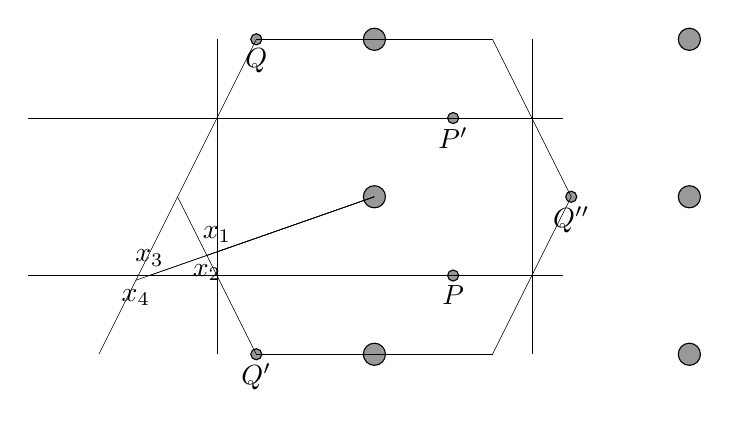
\begin{tikzpicture}[scale=2]
        \filldraw[fill=gray!80] (0,0) circle [radius=2pt]
                                (2,0) circle [radius=2pt]
                                (0,1) circle [radius=2pt]
                                (2,1) circle [radius=2pt]
                                (0,2) circle [radius=2pt]
                                (2,2) circle [radius=2pt];
        \filldraw[fill=gray!80] (0.5,0.5) circle [radius=1pt] node[anchor=north] {$P$}
                                (0.5,1.5) circle [radius=1pt] node[anchor=north] {$P'$}
                                (-0.75,2) circle [radius=1pt] node[anchor=north] {$Q$}
                                (-0.75,0) circle [radius=1pt] node[anchor=north] {$Q'$}
                                (1.25,1) circle [radius=1pt] node[anchor=north] {$Q''$};

        \draw[very thin] (-2.2,0.5) -- (1.2,0.5);
        \draw[very thin] (-1,0) -- (-1,2);
        \draw[very thin] (1,0) -- (1,2);
        \draw[very thin] (-2.2,1.5) -- (1.2,1.5);

        \draw[very thin] (-0.75,0) -- (0.75,0);
        \draw[very thin] (0.75,0) -- (1.25,1);
        \draw[very thin] (-0.75,0) -- (-1.25,1);
        \draw[very thin] (-0.75,2) -- (0.75,2);            
        \draw[very thin] (0.75,2) -- (1.25,1);
        \draw[very thin] (-0.75,2) -- (-1.75,0);
        %\draw[very thin] (0,1) -- (-2,0.3);

        \path [name path = l] (0,1) -- (-2,0.3);
        \path [name path = 1l] (-1,0) -- (-1,2);
        \path [name path = 2l] (-0.75,0) -- (-1.25,1);
        \path [name path = 3l] (-2.2,0.5) -- (1.2,0.5);
        \path [name path = 4l] (-0.75,2) -- (-1.75,0);

        \draw [name intersections = {of = l and 1l, by=x}]
                [very thin ] (0,1) -- (x) node[anchor=south] {$x_1$};
        \draw [name intersections = {of = l and 2l, by=x}]
                [very thin ] (0,1) -- (x) node[anchor=north] {$x_2$};
        \draw [name intersections = {of = l and 3l, by=x}]
                [very thin ] (0,1) -- (x) node[anchor=south] {$x_3$};
        \draw [name intersections = {of = l and 4l, by=x}]
                [very thin ] (0,1) -- (x) node[anchor=north] {$x_4$};
        %\draw (1,0) -- (3,0) -- (4,1.73) -- (3,3.46) -- (1,3.46) -- (0,1.73) -- cycle;
        %\draw[help lines] grid(5,5);
    \end{tikzpicture}
    \caption{二维长方倒格子的第一布里渊区和一些布拉格线的示意。}
    \label{二维长方倒格子的第一布里渊区和一些布拉格线的示意}
\end{figure}

            三维情况下,简并条件\autoref{简并微扰使用条件1}可以写作
            \begin{equation}
                |k|=|k-G_h|,
            \end{equation}
            相当于
            \begin{equation}
                k\cdot G_h=\frac{1}{2}G_h.
            \end{equation}
            也就是发生布拉格反射的劳厄条件。这说明,在电子波矢接近出现布拉格反射的区域时,弱周期势有明显作用,
            导致能隙的出现,因而准连续的$\varepsilon(k)$分裂成能带,这是晶体中电子结构重要的基本性质。金属、半导体的很多特性与此有关。

        \section{紧束缚近似}\label{section:紧束缚近似}
            
            本章换一角度,考虑将孤立原子放到布拉维格子的格点上,形成晶格时,单电子态发生的变化,为处理方便,仅讨论近邻原子的电子波函数相互交叠
            相当小,即电子紧束缚在原子上的情形,重在强调交叠引起的变化。本节的目的,除去从另一角度将\autoref{section:布洛赫定理及能带}的一般讨论具体
            化外,其物理图像及结果较适用于过渡族金属中的$3d$电子,及固体中的其他内层电子。

            \subsection{模型及计算}
                假定$\varphi_i(r)$是孤立原子与本征能量$\varepsilon_r$对应的单电子本征态,即
                \begin{equation}
                    \hat{H}_{at}\varphi_i=\left[ - \frac{\hbar^2}{2m} +V_{at}(r) \right]\varphi_i=\varepsilon_r\varphi_i,
                \end{equation}                
                其中$V_{at}(r)$是单原子势场,$i$代表原子中的某一量子态,假定$\varphi_i(r)$是归一化且不简并的。

                紧束缚近似的出发点是将晶体中单电子波函数看出是$N$(晶体中格点数)个简并的原子波函数的线性组合,及
                \begin{equation}
                    \psi(r)=\sum_{R_m}a_m\varphi_i(r-R_m)\label{紧束缚近似的假设基础},
                \end{equation}
                且近似的认为
                \begin{equation}
                    \int \varphi_i^*(r-R_n)\varphi_i(r-R_m)\dif r=\delta_{nm}\label{格点波函数的正交归一性},
                \end{equation}
                即同一格点上的$\varphi_i$归一,不同格点上的$\varphi_i$因为交叠很小而正交。

                \autoref{紧束缚近似的假设基础}中波函数的取法,相当于在每个格点附近,$\psi(r)$近似为该处原子波函数,此法也称为原子轨道线性组合法
                (Linear Combination of Atomic Orbitals,简称LCAO)即晶体中共有化的轨道由原子轨道$\varphi_i(r-R_m)$的线性组合构成。
                
                $\psi(r)$应为布洛赫波函数,这要求\autoref{紧束缚近似的假设基础}中
                \begin{equation}
                    a_m=\frac{1}{\sqrt{N}}e^{ik\cdot R_m}.
                \end{equation}
                这样,\autoref{紧束缚近似的假设基础}中的$\psi(r)$可以用波矢$k$标记,即
                \begin{equation}
                    \psi_k(r)=\frac{1}{\sqrt{N}}\sum_{R_m}e^{ik\cdot R_m}\varphi_i(r-R_m)\label{满足布洛赫定理的紧束缚近似波函数},
                \end{equation}
                将\autoref{满足布洛赫定理的紧束缚近似波函数}代入晶体中的薛定谔方程,得到
                \begin{equation}
                    \sum_{R_m}e^{ik\cdot R_m}\left[ - \frac{\hbar^2}{2m}\nabla^2 - \varepsilon(k)+V(r) \right]\varphi_i(r-R_m)=0.
                \end{equation}
                变换得
                \begin{equation}
                    \sum_{R_m}e^{ik\cdot R_m}\left[ \varepsilon_i-\varepsilon(k)+V(r)-V_{at}(r-R_m) \right]\varphi_i(r-Rm)=0.
                \end{equation}
                左称$\varphi_i^*(r)$并积分,并利用$\varphi_i$的正交归一性\autoref{格点波函数的正交归一性},得
                \begin{equation}
                    \begin{split}
                        \varepsilon_i&-\varepsilon(k)+\int\Delta V(r,0)\left|\varphi_i(r)\right|^2\dif r\\
                        &+\sum e^{ik\cdot R_m}\int\varphi_i^*(r)\Delta V(r,R_m)\varphi_i(r-R_m)\dif r=0,
                    \end{split}\label{归一化的紧束缚近似薛定谔方程}
                \end{equation}
                由此可以得到$\varepsilon(k)$,式中
                \begin{equation}
                    \Delta V(r,R_m)=V(r)-V_{at}(r-R_m),
                \end{equation}
                是晶格周期势和格点$R_m$处的原子势之差。

                利用\autoref{归一化的紧束缚近似薛定谔方程},
                \begin{equation}
                    \varepsilon(k)=\varepsilon_i-J(0)-\sum_{n. n.}J(R_m)e^{ik\cdot R_m}\label{紧束缚近似下的能级表示},
                \end{equation}
                式中$\sum_{n. n.}$表示求和仅涉及最近邻(nearest neighbours)项,
                \begin{equation}
                    -J(0)=\int\Delta V(r,0)\left|\varphi_i(r)\right|^2\dif r,
                \end{equation}
                $J(0)$一般大于零且数值不大,这是因为$\Delta V(r,0)$一般为负,且在$R_m=0$附近,
                $|\varphi_i(r)|^2$较大处,$\Delta V(r,0)$处接近于零,后面可以看到,这一项相当于能带的中心相对与原子能级
                $\varepsilon_i$有一小平移。
                \begin{equation}
                    -J(R_m)=\int\varphi_i^*(r)\Delta V(r,R_m)\varphi_i(r-R_m)\dif r\label{交叠积分},
                \end{equation}
                仅当相距为$R_m$的两格点上原子波函数有所交叠时才不为零,因而称为交叠积分或者重叠积分,在紧束缚近似下,只考虑最近邻的交叠。

                对于简单立方晶格中原子的$s$态,波函数$\varphi_s(r)$是球形对称的,对6个距离均为$a$的最近邻,交叠积分相同时取为$J_1$。
                同时,由于$s$态波函数具有偶宇称$\varphi_s(r)=\varphi_s(-r)$,因而$J_1>0$。将近邻格矢
                $(\pm a,0,0)$,$(0,\pm a,0)$,$(0,0,\pm a)$代入\autoref{紧束缚近似下的能级表示},得到
                \begin{equation}
                    \varepsilon(k)=\varepsilon_s-J_0-2J_1\left( \cos{k_xa}+\cos{k_ya}+\cos{k_za} \right)\label{紧束缚近似下的能带和格矢关系},
                \end{equation}
                其中$J_0$是$J(0)$的简写。

                由于最近邻原子的波函数的交叠,$N$重简并解除,展宽成能带,包含$N$个由不同$k$标记的扩展态。以
                简单立方晶格的$s$态为例,$\varepsilon_s$展成宽度为$12J_1$的能带。

                由于能带从原子能级演化而来,能带常用原子能级的量子数标记,如$3s$,$3p$或$3d$带等,原子的内层电子,如过渡族元素的$d$
                电子,其轨道波函数与最近邻交叠甚少,形成的能带较窄,比较确定,这种分类方法比较合适,外层电子的波函数相互交叠较多,相应的能带较宽,
                有时不同能带之间有所重叠,原子能级与能带之间对应比较复杂。

                %//TODO:Wannier function should be written here, but we don't use it right now.

        %\section{能带结构的计算}
                %//TODO:这一部分与材料计算相关,考试中并不出现,之后再补。
        \section{费米面和态密度}\label{section:费米面和态密度}
            在\autoref{chapter:金属自由电子气体模型}中,已经讨论过费米面\index{费米面},它的重要性在于仅只费米面附近的电子参与热激发\index{热激发}和输运过程\index{输运过程},
            本节将重点分析晶格势场的影响,再次讨论费米面及相关的态密度\index{态密度},这也是能带计算给出的主要结果。

            \subsection{高布里渊区}
                晶格周期场存在时,费米面仍然有很大的意义,在基态情况下,$k$空间中单电子中单电子占据态和非占据态的分界面,但在简约布里渊区中表示时,形状有时会很复杂。
                除第1布里渊区外,引入第2,第3等高布里渊区的概念有助于问题的讨论。

                第n个布里渊区的定义为从第$n-1$个布里渊区出发,只经过一个布拉格平面,所能到达的所有点的集合。

                除第1布里渊区\index{布里渊区!第1布里渊区}以外,高布里渊区\index{布里渊区!高布里渊区}均是有分立的小块组成,但是每个布里渊区的总体积相等,为倒空间一个原胞的体积。

            \subsection{费米面的构造}
                利用近自由电子近似,费米面总是与布里渊区边界垂直相交,如果晶体有和波矢$k$垂直的反映面,沿这一方向,$\varepsilon(k)$应是对称的,
                同时,$\varepsilon(k)$又是倒格子空间的周期函数,因而有
                \begin{align}
                    \varepsilon(k)=\varepsilon(-k),&\left( \frac{\partial\varepsilon}{\partial k} \right)_k=\left( \frac{\partial\varepsilon}{\partial k} \right)_{-k};\\
                    \varepsilon(k)=\varepsilon(k+G_h),&\left( \frac{\partial\varepsilon}{\partial k} \right)_k=\left( \frac{\partial\varepsilon}{\partial k} \right)_{k+G_h};\\
                \end{align}
                在布里渊区的边界上,$k=\pm G_h/2$,以上两式的结果不同
                \begin{align}
                    \left( \frac{\partial\varepsilon}{\partial k} \right)_{\frac{1}{2}G_h}&=-\left( \frac{\partial\varepsilon}{\partial k} \right)_{-\frac{1}{2}G_h},\\
                    \left( \frac{\partial\varepsilon}{\partial k} \right)_{\frac{1}{2}G_h}&=+ \left( \frac{\partial\varepsilon}{\partial k} \right)_{-\frac{1}{2}G_h}.
                \end{align}
                因此,在边界上$\left( \frac{\partial\varepsilon}{\partial k} \right)=0$。

            \subsection{态密度}
                在\autoref{section:模型和基态性质}中,已经对态密度有过定义,对于第$n$个能带的态密度$g_n(\varepsilon)$
                可以通过在$k$空间内第1布里渊区内,计算$\varepsilon\leq\varepsilon_n(k)\leq\varepsilon+\dif \varepsilon$等能面壳层的许可波矢来确定。
                假定$S_n(\varepsilon)$是等能面$\varepsilon_n(k)=\varepsilon$在第1布里渊区内的部分,$\dif S$是其上的面积元,$\delta k(k)$是在点$k$处等能面$S_n(\varepsilon)$和$S_n(\varepsilon+\dif\varepsilon)$
                之间的垂直距离,则
                \begin{equation}
                    g_n(\varepsilon)\dif \varepsilon=\frac{2}{V}\cdot\frac{V}{8\pi^3}\int_{S_n(\varepsilon)}^{}\delta k(k)\dif S\label{等能面壳层内的态密度}.
                \end{equation}
                因子2来源于每个$k$态可以容纳自旋取向相反的两个电子。由于
                \begin{equation}
                    \dif\varepsilon=\left|\nabla_k\varepsilon_n(k)\right|\delta k(k),
                \end{equation}
                代入\autoref{等能面壳层内的态密度}得到
                \begin{equation}
                    g_n(\varepsilon)=\int_{S_n(\varepsilon)}^{}\frac{1}{\left|\nabla_k\varepsilon_n(k)\right|}\frac{\dif S}{4\pi^3}\label{能带结构与态密度关系},
                \end{equation}
                由此,可以通过能带结构$\varepsilon_n(k)$计算态密度。

                $\varepsilon_n(k)$是倒格子的周期函数,因此,每个原胞中总有一些$k$值处于$|\nabla_k\varepsilon|=0$,这导致\autoref{能带结构与态密度关系}中被积函数的发散,虽然在三维情况可积
                但是斜率$\dif g_n(\varepsilon)/\dif \varepsilon$发散,$g_n(\varepsilon)$的这种奇异,称为Van Hove奇异\index{Van Hove奇异}

                假如在$k=0$处,$\nabla_k\varepsilon(k)=0$,则在这一点附近有
                \begin{equation}
                    \varepsilon=\varepsilon_0+a_1k_x^2+a_2k_y^2+a_3k_z^3,
                \end{equation}
                可以分为四种情况
                \begin{itemize}
                    \item[1] $a_1,a_2,a_3>0$,$\varepsilon(k)$在$k=0$处为极小;
                    \item[2] $a_1,a_2,a_3<0$,$\varepsilon(k)$在$k=0$处为极大;
                    \item[3] $a_1,a_2>0,a_3<0$,$\varepsilon(k)$有第一类鞍点;
                    \item[4] $a_1,a_2<0,a_3>0$,$\varepsilon(k)$有第二类鞍点;
                \end{itemize}
                %//TODO:这里四种情况的示意图还要画。
\chapter{能带论II}
    本章讨论布洛赫电子的动力学行为,将自由电子论的准经典模型推广为半经典模型\index{半经典模型}。
    引入有效质量、空穴等重要概念,并从能带论的角度讲述金属半导体和绝缘体的区别。

    \section{电子运动的半经典模型}
        处于布洛赫态
        \begin{equation}
            \psi_{nk}(r)=e^{ik\cdot r}u_{nk}(r)
        \end{equation}
        的电子的平均速度
        \begin{equation}
            \begin{split}
            \bar{v}_n(k)&=\frac{1}{m}\braket{\psi_{nk}^*(r)|\hat{p}|\psi_{nk}(r) }\\
                &=\frac{1}{m}\int u_{nk}^*(r)(\hat{p}+\hbar k)u_{nk}(r)\dif r.
            \end{split}
        \end{equation}
        根据\autoref{布洛赫形式的单电子薛定谔方程}
        \begin{equation}
            \hat{H}_k=\frac{\left( \hat{p}+\hbar k \right)^2}{2m}+V(r),        
        \end{equation}
        由于$k$值准连续,对薛定谔方程取$\nabla_k=\frac{\partial}{\partial k}$,得
        \begin{equation}
            \frac{\hbar}{m}(\hat{p}+\hbar k)u_{nk}(r)+\hat{H}_k\nabla_k u_{nk}(r)=\left[ \nabla_k \varepsilon_n(k)\right]u_{nk}(r)+\varepsilon_n(k)\nabla_ku_{nk}(r).
        \end{equation}
        右乘$u^*_{nk}(r)$再对$r$积分得到
        \begin{equation}
            \begin{split}
            \frac{\hbar}{m}\int u^*_{nk}(r)(\hat{p}&+\hbar k)u_{nk}(r)\dif r+\int u^*_{nk}(r)\hat{H}_k\nabla_k u_{nk}(r)\dif r\\
            &=\left[ \nabla_k \varepsilon_n(k)\right]\int u^*_{nk}(r)u_{nk}(r)\dif r+\varepsilon_n(k)\int u^*_{nk}(r)\nabla_k u_{nk}(r)\dif r.
            \end{split}
        \end{equation}
        由于算符$\hat{H}_k$的厄密性,是的等式左右第二相相消,再根据波函数的归一性,是的等式右边的第一项为1,等式左边积分为$\hbar v_n(k)$,因此有
        \begin{equation}
            v_n(k)=\frac{1}{\hbar}\nabla_k\varepsilon_n(k)\label{布洛赫态电子的平均速度}.
        \end{equation}

        \autoref{布洛赫态电子的平均速度}是一个非常值得注意的结果,由于布洛赫态是与时间无关的定态,尽管电子和周期排列的粒子实存在相互作用,但是其平均速度将永远保持,不会衰减,换言之,一个理想的晶体金属,将有无穷大的电导。

        但是由于晶体结构存在杂质缺陷,同时离子实有以平衡位置为中心的热运动,电子总会受到散射。因此关于电子的运动有两个方面的问题
        \begin{itemize}
            \item[1] 散射产生的原因和性质,
            \item[2] 两次散射之间布洛赫电子的运动。
        \end{itemize}
        电子运动的半经典模型主要回答第二个问题。

        \subsection{模型的表述}
            半经典模型\index{半经典模型}对外电场、磁场用经典的方式处理,对晶格周期场沿用能带论量子力学的处理方式,具体表述如下:
            
            每个电子具有确定的位置$r$,波矢$k$和能带指标$n$,对于给定的$\varepsilon_n(k)$,在外电场$E(r,t)$和
            外磁场$B(r,t)$作用下,位置、波矢、能带指标随时间的变化遵从如下规则:
            \begin{itemize}
                \item[1] 能带指标$n$是运动阐述,电子总处于同一能带中,忽略跃迁的可能性;
                \item[2] 电子的速度为
                            \begin{equation}
                                \dot{r}=v_n(k)=\frac{1}{\hbar}\nabla_k\varepsilon_n(k)\label{外场中半经典模型的电子速度};
                            \end{equation}
                \item[3] 波矢$k$随时间的变化为
                            \begin{equation}
                                \hbar\dot{k}=-e\left[ E(r,t)+v_n(k)\times B(r,t) \right]\label{外电磁场下波矢$k$随时间的变化}.
                            \end{equation}
            \end{itemize}
            
            在半经典模型中,波矢$k$和$k+G_h$仍是等价的,$\hbar k$如\autoref{subsection:波矢k的取值和物理意义}所述,是电子的晶体动量。

            \autoref{外场中半经典模型的电子速度}和\autoref{外电磁场下波矢$k$随时间的变化}是电子的运动方程,是晶格周期场的量子力学处理的结果全都概括在
            $\varepsilon_n(k)$中,半经典模型使能带结构与输运性质,即电子对外场的响应相联系,提供了能带结构推断输运性质或反过来从输运性质的测量结果推断能带结构的理论基础。

            对于模型的有效性,此处暂时不作证明。

        \subsection{有效质量}
            从\autoref{外场中半经典模型的电子速度}和\autoref{外电磁场下波矢$k$随时间的变化}出发,可以计算电子的加速度
            \begin{equation}
                \begin{split}
                    \dot{v}&=\frac{\partial}{\partial t}\left[ \frac{1}{\hbar}\nabla_k\varepsilon(k) \right]\\
                    &=\frac{1}{\hbar}\nabla_k\left[ \frac{1}{\hbar}\nabla_k\varepsilon(k) \right]\frac{\hbar\partial k}{\partial t}\\
                    &=\frac{1}{\hbar^2}\nabla_k\nabla_k\varepsilon(k)\cdot F_{\mathrm{ext}}.
                \end{split}\label{半经典模型中计算电子的加速度}
            \end{equation}
            此处省略能带指标,并用$F_{\mathrm{ext}}$代表作用在电子上的外电磁场力,和牛顿方程$m\dot{v}=F$相比,可以引入电子的有效质量\index{半经典模型!有效质量},
            或是有效质量张量\index{半经典模型!有效质量!有效质量张量}
            \begin{equation}
                \left[ \frac{1}{m^*} \right]_{ij}=\frac{1}{\hbar^2}\frac{\partial\varepsilon_n(k)}{\partial k_i\partial k_j}.
            \end{equation}
            由于微商可以交换次序,这时对称张量,晶体的点群对称性可以使张量的独立分量数减少\footnote{见阎守胜书2.2.6节《点群对称性和晶体的物理性质》。}。
            通常用通过选择坐标轴于主轴方向,使之对角化的方式来达到。设$k_x$,$k_y$,$k_z$轴为主轴,
            \begin{equation}
                \frac{1}{m^*}=\frac{1}{\hbar}\frac{\partial^2\varepsilon_n(k)}{\partial k^2_{\alpha}},\alpha=x,y,z\label{有效质量定义}.
            \end{equation}

            有效质量的作用在于它概括了晶格内部周期场的作用,可以能简单地有外场里决定电子的加速度。

            对于简单立方晶体紧束缚近似下的$s$ 能带,\autoref{紧束缚近似下的能带和格矢关系}按照有效质量的定义,可以算出在能带底,即$k=(0,0,0)$点,有效质量张量
            约化为一标量,
            \begin{equation}
                m_x^*=m_y^*=m_z^*=m^*=\frac{\hbar^2}{2aJ_1},
            \end{equation}
            为正值,在能带底,即$k=\left( \pm\frac{\pi}{a},\pm\frac{\pi}{a},\pm\frac{\pi}{a} \right)$点
            \begin{equation}
                m_x^*=m_y^*=m_z^*=m^*=-\frac{\hbar^2}{2aJ_1},
            \end{equation}
            为负值。在能带底和能带顶,有效质量的各向同性来源于晶格的立方对称性,但在能带第附近,有效质量为正,能带顶附近,有效质量为负,具有普遍性,因为能带第和能带顶分别对应于
            $\varepsilon_n(k)$函数的极小或极大,具有正值或者负值的二级微商。

            一般来讲,对于宽的能带,能量随波矢$k$的变化较为剧烈,有效质量小,而对于窄的能带,应有大一些的有效质量,从紧束缚近似的角度,后者相当于相邻原子电子波函数交叠甚少,相对而言,
            定域性更强一些。

            知道材料的能带结构,可以按定义计算有效质量,实际工作中,常通过电子比热系数确定有效质量
            \begin{equation}
                \frac{\gamma_{exp}}{\gamma_0}=\frac{m^*}{m},
            \end{equation}
            其中$\gamma_0$是自由电子气体的热容理论值,$\gamma_{exp}$是实验测量值,这是由于$\gamma$比例与费米面的态密度$g(\varepsilon_F)$,
            而后者比例于电子质量,有时称为热有效质量。

    \section{恒定电场、磁场作用下电子的运动}
        \subsection{恒定电场作用下的电子}\label{subsection:恒定电场作用下的电子}
            在恒定电场$E$的作用下,半经典运动方程\autoref{外电磁场下波矢$k$随时间的变化}简化为
            \begin{equation}
                \hbar\dot{k}=-eE,
            \end{equation}
            其解为
            \begin{equation}
                k(t)=k(0)-\frac{eEt}{\hbar},
            \end{equation}
            即每个电子的波矢$k$均以同一速率发生改变。

            对于自由电子,如电场使$k$增加,由于$\hbar k$是电子的动量,电子将不断被加速,实际上,因为受到散射,这种加速是有限的。

            布洛赫电子的行为则完全不同,
            \begin{figure}[ht]
    \centering
    \subfloat[电子能量]
    {
        \begin{tikzpicture}{scale=0.3}
                \begin{axis}
                    [
                    axis lines=center,
                    xlabel={$\vec{k}$},
                    ylabel={$\varepsilon$},
                    ymax=2,ymin=0,
                    ytick=\empty,
                    xtick=\empty,
                    ]
                        \addplot[red,domain=-3.14:3.14,samples=200] {1-cos(deg(x))};
                \end{axis}
                
        \end{tikzpicture}%     
    }
    \\
    \subfloat[电子速度]
    {
        \begin{tikzpicture}{scale=0.3}
            \begin{axis}
                [
                axis lines=center,
                xlabel={$\vec{k}$},
                ylabel={$v$},
                ymax=1,ymin=-1,
                ytick=\empty,
                xtick=\empty,
                ]
                    \addplot[red,domain=-3.14:3.14,samples=200] {sin(deg(x))};
            \end{axis}
    \end{tikzpicture}%
    }   
    \\
    \subfloat[有效质量]
    {
        \begin{tikzpicture}{scale=0.3}
                \begin{axis}
                    [
                    axis lines=center,
                    xlabel={$\vec{k}$},
                    ylabel={$\varepsilon$},
                    ymax=2,ymin=0,
                    ytick=\empty,
                    xtick=\empty,
                    ]
                        \addplot[red,domain=-3.14:3.14,samples=200] {1-cos(deg(x))};
                \end{axis}
                
        \end{tikzpicture}%     
    }
    \caption{能带速度有效质量和波矢关系。}
    \label{能带速度有效质量和波矢关系}
\end{figure}
            \autoref{能带速度有效质量和波矢关系}给出一个一维能带$\varepsilon(k)$,以及相应的$v(k)$和$m^*(k)$的示意图,如果电场方向使$k$
            不断增加,在$k=0$附近,$\varepsilon(k)\propto k^2$,$v(k)\propto k$,同时$m^*>0$,类似于自由电子,电子被加速,但在接近布里渊区边界,
            速度达到极大值后,$m^*<0$,$k$增加时速度反而减小,以致于电子的加速度方向与电场力方向相反,这种特别的行为实际上是晶格周期场的作用,使电子在布里渊区
            边界受到布拉格反射的结果。在半经典模型中,这种晶格场力隐含在$\varepsilon(k)$函数中。

            当电子到达区边界后,在电场作用下,$k$继续增加,将进入第二布里渊区,在简约布里渊区图示中,这等价于再次进入第一布里渊区。
            电子在$k$空间的循环运动,相应的速度随时间在$\pm v_{max}$之间周期性变化,意味着电子在实空间位置的振荡,直流的外加电场可能产生交变的电流,
            这种效应称为布洛赫振荡\index{布洛赫振荡}。实际上,由于散射的存在,两次散射间电子在$k$空间移动的距离与布里渊区尺度相比甚小,一般情况下难以观察到。

        \subsection{满带不导电}
            能带中每个电子对电流密度的贡献为$-ev(k)$,带中所以电子的贡献为
            \begin{equation}
                J=(-e)\int_{\mathrm{occ}}v(k)\frac{\dif k}{4\pi^3}\label{能带中所有电子对电流密度的贡献},
            \end{equation}
            其中occ表示占据态积分,由于$\varepsilon_n(k)$函数的对称性,$\varepsilon_n(k)=\varepsilon_n(-k)$,根据\autoref{外场中半经典模型的电子速度}可知,
            \begin{equation}
                v_n(k)=-v_n(-k),
            \end{equation}
            即处在$k$态和$-k$态的电子,对电流密度的贡献恰好相消。对于填满的能带,外加电场时,每个电子的波矢$k$随时间变化,但如\autoref{subsection:恒定电场作用下的电子}
            所述,由于$k$与$k+G_h$等价,满带的状况并不改变,因而$j=0$,即满带电子不参与导电,电导仅来源于部分填满的能带中电子的贡献,在外加电场和电子所受散射的共同作用下,电子对给定未满能带在$k$
            空间的占据态是非对称的,对总电流的贡献不能完全抵消。
        
        \subsection{近满带中的空穴}
            对于仅仅电子占满的近满带,对电流密度的贡献同样由\autoref{能带中所有电子对电流密度的贡献}式给出,利用满带不导电的事实,有
            \begin{equation}
                J+(-e)\int_{\mathrm{unocc}}^{}v(k)\frac{\dif k}{4\pi^3}=0,
            \end{equation}
            其中下标unocc表示积分只涉及未占据态\index{未占据态},这样近满带对电流密度的贡献可以等价地写为
            \begin{equation}
                J=e\int_{\mathrm{unocc}}^{}v(k)\frac{\dif k}{4\pi^3}.                
            \end{equation}
            相当于所有的带脑子占据态看成是空态,而所有的未占据态看作是电荷为$+e$的粒子所占据,因此,尽管电荷仅被电子传输,但可以
            引入一种假象的,带正电荷$e$填满带中所有电子未占据态的粒子,这种假象的粒子,称为空穴\index{空穴}。对于近满带,带中大量电子的行为可简化为
            成少数空穴的效应,这样是十分方便的。

            在外加电磁场中,未占据态的运动应个周围的占据态相同,同样用半经典模型描述,\autoref{半经典模型中计算电子的加速度}可以写作
            \begin{equation}
                \dot{v}_n(k)=\frac{1}{m^*}(-e)[E+ v_n(k)\times B].
            \end{equation}
            由于未占据态一般在带顶,带顶附近,$m^*$有负值,上式等价为
            \begin{equation}
                \dot{v}_n(k)=\frac{1}{|m^*|}e\left[ E+v_n(k)\times B \right],
            \end{equation}
            这相当于在近满带顶的空穴,带有正电荷$e$,且有正的有效质量$m^*_h=|m^*|$,速度仍为$v_n(k)$。

            注意,对于某一固定能带,如认为电流为空穴所携带,则应把电子的占据态,电子没有贡献,如认为电流来源于占据态上的电子,则空穴没有
            贡献,但对于不同的能带,可以对某些带用电子的图象,另外一些用空穴的图像,取决于哪一种更为方便。

            空穴的引入,立即解决了自由电子其他模型在解释某些金属等正霍尔系数时所遇到的困难(\ce{Be},\ce{Zn},\ce{Cd}等),从能带论的角度,带正电荷的载流子的存在易于理解,在半导体中
            长碰到价带顶的空穴,在半金属中,由于能带交叠,同时有空穴、电子存在,对于他们的了解,空穴的概念非常重要。

        %\subsection{导体,半导体和绝缘体的能带论解释}
        \subsection{恒定磁场作用下电子的准经典运动}
            只有恒定的均匀磁场存在时,半经典方程为
            \begin{align}
                \dot{r}&=v(k)-\frac{1}{\hbar}\nabla_k\varepsilon(k)\label{恒定磁场下速度与波矢关系},\\
                \hbar\dot{k}&=(-e)v(k)\times B\label{恒定磁场下波矢变化与磁场关系}.
            \end{align}
            可以看出,在$k$空间中,波矢$k$的变化总是
            \begin{itemize}
                \item[1] 垂直于$B$的方向,假定$B$在$z$方向,从\autoref{恒定磁场下波矢变化与磁场关系}得$\hbar \dot{k}\cdot B=0$,即$\dif k_z/\dif t=0$,$k)z$保持为常量;
                \item[2] 垂直于$v$的方向,即$\hbar\dot{k}\cdot v(k)=0$,即$\dif \varepsilon(k)/\dif t=0$。
            \end{itemize}

            因此,电子总是沿着垂直与$B$的平面和等能面的交线运动,对于自由电子,等能面为球形,轨道为圆,如带脑子不受散射,圆周运动的周期
            \begin{equation}
                T=\frac{\oint\dif k}{\dif k/\dif t}=\frac{2\pi\hbar k}{evB}=\frac{2\pi m}{eB}\label{磁场下电子圆周运动的周期},
            \end{equation}
            角频率为
            \begin{equation}
                \omega_c=\frac{2\pi}{T}=\frac{eB}{m},
            \end{equation}
            通常称为回旋频率\index{回旋频率},对于布洛赫电子,闭合轨道并非一定是圆形,形式上可以写成
            \begin{equation}
                \omega_c=\frac{eB}{m^\prime_c}\label{回旋频率与回旋有效质量},
            \end{equation}
            其中$m^\prime_c$称为回旋有效质量\index{回旋有效质量},类似于\autoref{磁场下电子圆周运动的周期},有
            \begin{equation}
                T(\varepsilon,k_z)=\frac{2\pi}{\omega_c}=\oint\frac{\dif k}{|\dot{k}|}=\frac{\hbar}{eB}\oint\frac{\dif k}{|v_\perp|}\label{电子在此磁场运动周期改写1},
            \end{equation}
            其中$v_\perp$是电子速度在磁场垂直方向的分量,假定$\Delta (k)$是在轨道平面上在$k$点与轨道垂直并连接$k$点和同一平面上能量为
            $\varepsilon+\Delta\varepsilon$的等能轨道的矢量,由于$\Delta (k)$与$v_\perp$处于同一方向,根据\autoref{恒定磁场下速度与波矢关系}有
            \begin{equation}
                \Delta \varepsilon=\hbar|v_\perp|\Delta(k)
            \end{equation}
            \autoref{电子在此磁场运动周期改写1}可以改写为
            \begin{equation}
                \frac{2\pi}{\omega_c}=\frac{\hbar^2}{eB}\oint\frac{\Delta(k)\dif k}{\Delta\varepsilon}=\frac{\hbar^2}{eB}\frac{\partial}{\partial\varepsilon}A(\varepsilon,k_z),
            \end{equation}
            $A(\varepsilon,k_z)$是用$\varepsilon$,$k_z$标记的轨道在$k$空间位处的面积,而$\oint\Delta(k)\dif k$正是
            $A(\varepsilon+\Delta\varepsilon,k_z)-A(\varepsilon,k_z)$,与\autoref{回旋频率与回旋有效质量}相比,
            \begin{equation}
                m_c^*=\frac{\hbar^2}{2\pi}\frac{\partial}{\partial\varepsilon}A(\varepsilon,k_z).
            \end{equation}
            此处的质量与之前所说的有效质量不一定相同,$m^*_c$是一个轨道的性质,并不单纯地只与一个特定的电子态相关联。

            用磁场方向的单位矢量$\hat{B}$叉乘\autoref{恒定磁场下波矢变化与磁场关系},得到
            \begin{equation}
                \frac{\dif}{\dif t}r_\perp=-\frac{\hbar}{eB}\hat{B}\times\frac{\dif }{\dif t}k,
            \end{equation}
            其中$r_\perp$是电子在实空间位置矢量在垂直磁场方向的投影,积分后得到
            \begin{equation}
                r_\perp(t)=r_\perp(0)=-\frac{\hbar}{eB}\times[k(t)-k(0)].
            \end{equation}
            因此,电子在实空间的位置矢量可由在$k$空间的轨道绕磁场轴旋转\ang{90},并乘以因子$\hbar/eB$得到,
            如果电子在$k$空间做回旋运动,则在实空间也做回旋运动,磁场越强,轨道半径越小。

            沿磁场方向($z$方向),有
            \begin{equation}
                z(t)=z(0)+\int_{0}^{t}v_z(t)\dif t, v_z=\frac{1}{\hbar}\frac{\partial}{\partial k_z},
            \end{equation}
            对自由电子,$v_k$为常数,沿磁场方向作匀速直线运动,对布洛赫电子,尽管$k_z$固定,但$v_z$未必一定不变,运动不一定是匀速的。
        
    \section{费米面的测量}
        金属材料中的物理过程主要有费米面附近电子的行为决定,因此费米面的实验测定非常重要,关于费米面的几何知识,主要来源于
        基于德哈斯-范阿尔芬效应\index{德哈斯-范阿尔芬效应}的实验,这是本机讨论的重点,效应色剂磁场作用下在晶格周期场中的布洛赫电子,
        严格地应从薛定谔方程出发,但是由于求解比较困难,这里线给出磁场中自由电子的结果,有助于理解布洛赫电子的结果。
        \subsection{均匀磁场中的自由电子}
            对于边长为$L$,分别平行与$x$,$y$,$z$轴的立方体中的电子,在沿$z$方向均匀磁场$B$的情况下,本征能量由量子数$v$和$k_z$决定:
            \begin{equation}
                \varepsilon(k_z,v)=\frac{\hbar^2}{2m}k_z^2+\left( v+\frac{1}{2} \right)\hbar\omega_c, v=0,1,2\cdots\label{均匀磁场下电子运动的本征值}
            \end{equation}
            其中,$\omega_c$为\autoref{回旋频率与回旋有效质量}的回旋频率,$k_z$取值与吴磁场时相同,
            \begin{equation}
                k_z=\frac{2\pi}{L}n_z, n_z\text{为整数。}
            \end{equation}
            这与电子沿磁场方方向(z方向)运动,洛伦兹力为零,能量不改变的事实相符\footnote{为了处理简单,本征能量忽略了电子自旋和此处的相互作用能。}。

            在垂直于磁场的方向,无磁场时的动能$\hbar^2(k_x^2+k_y^2)/2m$,按\autoref{均匀磁场下电子运动的本征值},将$\hbar\omega_c$为单位量子化,简并到朗道能级\index{朗道能级}
            $\left( v+\frac{1}{2} \right)\hbar\omega_c$上,这样,在$k$空间中,许可态的代表点将简并到朗道管\index{朗道管}上,其截面为朗道环\index{朗道管!朗道环}。

            相邻两个朗道环间的面积为
            \begin{equation}
                \Delta A =\pi\Delta(k_x^2+k_y^2)=\frac{2\pi m\Delta\varepsilon}{\hbar^2}=\frac{2\pi m\hbar\omega_c}{\hbar^2}=\frac{2\pi eB}{\hbar},
            \end{equation}
            是一个正比于外加磁场$B$的常量,在$k_z$固定的平面中,态密度为$L^2/4\pi^2$,每个朗道能级,或朗道环上的简并度为
            \begin{equation}
                p=\frac{2e}{h}BL^2,
            \end{equation}
            在\SI{1}{\tesla}下,对于$L=\SI{1}{\cm}$的样品,简并度约为$10^{11}$,每个朗道能级都是高度简并的。
        \subsection{布洛赫电子量子化}
            对于布洛赫电子,电子的半经典闭合轨道将按玻尔量子化条件,即
            \begin{equation}
                \oint p\cdot\dif r=(v+\gamma)2\pi\hbar\label{半经典闭合轨道的量子化},
            \end{equation}
            量子化,其中$v$为整数,$\gamma$是一相位常数,典型值为$1/2$,按照半经典模型,\autoref{半经典闭合轨道的量子化}
        \subsection{德哈斯-范阿尔芬效应}
        
\chapter{晶格振动}
    在之前的单电子近似以及紧束缚近似等研究方法中都认为离子实是保持静止不动的,
    因此也得出了一些与实际不符结果,比如理想周期势中,电子的运动不受散射,相应的电导和热导
    也是无穷大,实际上离子实围绕其平衡位置发生热振动导致晶格对理想周期势的偏离,
    这是金属中电子所受散射的主要来源,导致金属电导随温度的变化。

    本章相当于在之前的电子薛定谔方程上叠加晶格的薛定谔方程,形成多体问题。但是利用晶格振动很小这一事实
    可以对晶格离子实之间作用能进行级数展开,并保留第一个非零项(2次项),这种做法称为简谐近似\index{简谐近似},
    在经典力学中,简谐近似下的小振动有精确解,而在量子力学中,可以通过将其量子化来解决。

    本章的内容从简谐晶体的经典运动讨论,建立离子实的运动方程,得到晶格振动的简正模(normal mode)\index{简正模}
    的能量和频率。然后对简谐晶体的量子力学处理,强调了引进简正坐标将多体问题化为单体问题的方法,并建立了声子的概念,
    在此基础上讨论了晶格系统的平衡态性质下的晶格比热以及相关的近似模型。有关晶格振动谱是实验测定以及离子实作用能中
    高次项对运动的影响,也就是非简谐项,主要涉及晶体的热膨胀和热导率。

    \section{晶体的经典运动}
        前面的章节中,假定晶体中离子实不动,并且周期性规则排列,其结构用布拉维格子和基元
        来描述,本章将采用更实际的物理图像:
        \begin{itemize}
            \item[1] 仍然假定晶体中离子实可以有布拉维格子的格式$R_n$来标记,但是是平衡位置,原因在于离子实不再静止但是实验观察表面,布拉维格子依然存在;
            \item[2] 离子实微扰平衡位置做小的振动,其瞬时位置对平衡位置的偏离小于离子间距,如之前所述,这简化了晶格振动的理论处理。
        \end{itemize}
        \subsection{简谐近似}
            假定晶体中离子实或原子任意时刻的位置为
            \begin{equation}
                R(R_n)=R_n+u(R_n),
            \end{equation}
            其中$u(R_n)$是对平衡位置$R_n$的偏离。

            如果将两个原子之间的相互作用势能写出$\Phi[R(R_n)-R(R_{n^{\prime}})]$,晶体的
            总势能为
            \begin{equation}
                \begin{aligned}
                    V&=\frac{1}{2}\sum{}^{\prime}_{R_n,R_{n^\prime}}\Phi[R(R_n)-R(R_{n^{\prime}})]\\
                    &=\frac{1}{2}\sum{}^{\prime}_{R_n,R_{n^\prime}}\Phi[R_n-R_{n^{\prime}}+u(R_n)-u(R_{n^{\prime}})].
                \end{aligned}
            \end{equation}
            由于$\left\vert u(R_n)-u(R_{n^\prime})\right\vert\leq\left\vert R_n-R_{n^{\prime}}\right\vert$,可将相互作用
            势能在其平均值作泰勒展开为
            \begin{equation}
                \begin{aligned}
                    V=&\frac{1}{2}\sum{}^{\prime}_{R_n,R_{n^\prime}}\Phi(R_n-R_{n^\prime})\\
                    &+\frac{1}{2}\sum{}^{\prime}_{R_n,R_{n^\prime}}[u(R_n)-u(R_{n^\prime})]\cdot\nabla\Phi(R_n-R_{n^\prime})\\
                    &+\frac{1}{4}\sum{}^{\prime}_{R_n,R_{n^\prime}}[u(R_n)-u(R_{n^\prime})]\cdot\nabla^2\Phi(R_n-R_{n'})+\cdots
                \end{aligned}\label{对离子实相互作用势的泰勒展开}
            \end{equation}
            上式右边第一项,是晶体中每个原子都处在平衡位置时的相互作用能,这是一个常数,在讨论动力学问题时一般不考虑,
            第二项,及位移的线性项,由于原子处于平衡位置对应于相互作用能的极值二消失。对于平衡势能第一个非零的改正项
            是位移的二次项,在总势能中仅保留这一项称为简谐近似,在直角坐标系中写作分量的形式
            \begin{equation}
                V=\frac{1}{4}\sum{}^{\prime}_{R_n,R_{n^\prime}}[u_\mu(R_n)-u_\mu(R_{n^\prime})]\Phi_{\mu v}(R_n-R_{n'})\times[u_v(R_n)-u_v(R_{n^\prime})]\label{简谐近似的相互作用能},
            \end{equation}
            其中,$\mu,v=x,y,z$,而
            \begin{equation}
                \Phi_{\mu v}(r)=\frac{\partial^2\Phi(r)}{\partial r_\mu\partial r_v},
            \end{equation}
            在\autoref{对离子实相互作用势的泰勒展开}中,对平衡势能的其他修正项,主要是位移的3次项和4次项,
            称为非简谐项,对于热传导和热膨胀物理现象的解释,非简谐项非常重要。


        \subsection{一维单原子链,声学支}
            尽管相互作用中只保留简谐项的简单晶体的晶格振动可用经典力学处理,这里先研究最简单的每个晶胞只有一个
            但原子链,避免三维情形的复杂性,更为注意问题的物理方面。

            假定一维单原子链中每个原子质量为$M$,布拉维格子的格矢$R_n=na$,总长为$L=Na$,$N$为原胞总数,$a$为格点间距,
            链上任意原子的运动方程为
            \begin{equation}
                M\ddot{u}(na)=-\frac{\partial V}{\partial u(na)}\label{经典条件一维原子链的离子实运动方程1},
            \end{equation}
            其中$u(na)$为以$na$为中心振动的原子在沿链方向对其平衡位置的偏离。

            为简单起见,仅考虑最近邻原子间的相互作用,\autoref{简谐近似的相互作用能}变为
            \begin{equation}
                \begin{aligned}
                    V&=\frac{1}{4}\sum{}^{\prime}_{R_n,R_{n^\prime}}[u_\mu(R_n)-u_\mu(R_{n^\prime})]^2\Phi_{xx}(R_n-R_{n'})\\
                    &=\frac{1}{2}\sum_{n}\beta\left[ u(na)-u((n+1)a) \right]^2,
                \end{aligned}\label{只考虑最近邻的离子实简谐相互作用势}
            \end{equation}
            其中
            \begin{equation}
                \beta=\Phi_{xx}(a)=\frac{\dif^2\Phi(x)}{\dif x^2}.
            \end{equation}
            \autoref{只考虑最近邻的离子实简谐相互作用势}中系数变为$\frac{1}{2}$的原因是,求和方式发生了变化,没有对任意一对相互作用势
            重复计算。

            \autoref{只考虑最近邻的离子实简谐相互作用势}代入\autoref{经典条件一维原子链的离子实运动方程1},运动方程为
            \begin{equation}
                M\ddot{u}(na)=\beta\left[ u((n+1)a)+u((n-1)a)-2u(na) \right]\label{经典条件一维原子链的离子实运动方程2},
            \end{equation}
            这是原子之间用力常数为$\beta$的无质量弹簧连接起来的链的运动方程,利用数理方程知识,该方程的解
            应为波的形式,由于运动方程有平移不变性,解应该满足布洛赫定离,即每一解均有特定波矢$q$标记,根据\autoref{布洛赫定理},
            可以写作
            \begin{equation}
                u(na,t)=e^{iqna}u(0,t)\label{简谐近似下的离子实运动公式},
            \end{equation}
            这里按照习惯将晶格振动的波矢取成$q$,以和电子的波矢$k$相区别,两者都是同一倒格子空间中的矢量。

            \autoref{简谐近似下的离子实运动公式}说明各个原胞中原子的振幅相等,并有按$e^{iqna}$变化的一定的相位关系,
            这样,每确定$q$的解代表波长为$2\pi/|q|$的集体运动,称为格波,也成为晶格振动的一个简正模,或是简正模式,
            令$u(0,t)$取$Ae^{-iat}$的形式,\autoref{简谐近似下的离子实运动公式}也就可以写作
            \begin{equation}
                u(na,t)=Ae^{i(qna-qt)}.
            \end{equation}
            代入运动方程\autoref{经典条件一维原子链的离子实运动方程2},得到
            \begin{equation}
                \begin{aligned}
                    -M\omega^2Ae^{i(qna-qt)}&=-\beta[2-e^{-iqa}-e^{iqa}]Ae^{i(qna-qt)}\\
                    &=-2\beta[1-\cos{qa}]Ae^{i(qna-qt)},
                \end{aligned}
            \end{equation}
            也就是说,对于特定的$q$,相应的频率为
            \begin{equation}
                \omega(q)=\sqrt{\frac{2\beta(1-\cos{qa})}{M}}=2\sqrt{\frac{\beta}{M}}\left\vert \sin{\frac{1}{2}qa}\right\vert,
            \end{equation}
            这就是格波的色散关系,取正根的原因是物理上讲频率为实数。

            $q$的取值根据周期性边界条件\autoref{周期性边界条件}确定,这要求
            \begin{equation}
                e^{iqNa}=1,
            \end{equation}
            相当于
            \begin{equation}
                q=\frac{l}{N}\frac{2\pi}{a},l=\pm1,\pm2,\cdots
            \end{equation}
            因此,在$q$空间中,许可波矢的态密度为$L/2\pi$,不等价的$q$限制在第一布里渊区中,
            由于布里渊区的尺度为$\frac{2\pi}{a}$,所以$q$的数目与晶胞数相同,
            \begin{figure}[ht]
    \centering
    \begin{tikzpicture}
        \begin{axis}[
            xmin=-1.6,xmax=1.6,
            ymin=0,ymax=1.3,
            xlabel={$q$},
            ylabel={$\omega(q)$},
        ]
            \addplot[domain=0:1.57,samples=100] {sin(deg(x)};
            \addplot[pos=0,domain=-1.57:0] {sin(-deg(x)};
           % node (0,1) {$2\sqrt{\frac{\beta}{M}}$};
        \end{axis}
    \end{tikzpicture}
    \caption{仅考虑最近邻相互作用的单原子链的色散关系。}
    \label{仅考虑最近邻相互作用的单原子链的色散关系}
\end{figure}
        \subsection{一维双原子链,光学支}
        \subsection{三维情形}
    \section{简谐晶体的量子理论}
        \subsection{简正坐标}
        \subsection{声子}
        \subsection{晶格比热}
        \subsection{声子态密度(声子模式密度)}
    \section{晶格振动谱的实验测定}
        \subsection{中子的非弹性散射}
        \subsection{可见光的非弹性散射}
    \section{非简谐效应}
        \subsection{热膨胀}
        \subsection{晶格热导率}
\chapter{Problems}
\section{能带理论}
内容来自课后习题和习题课。
\subsection{量子力学基础}
    该题来源于黄昆书P582.
    \begin{example}
        根据$k=\pm \frac{\pi}{a}$状态\textbf{简并微扰}结果,求出与$E_+$、$E_-$对应的本征态波函数$\psi_+$和$\psi_-$,说明他们都代表驻波
        并比较两个电子云分布(即$|\psi|^2$),说明能隙的来源,假设($V_n=V_n^*$)。

        根据题意可知,该体系存在二重简并,波函数$\psi$可视为两简并态叠加
        \begin{equation*}
            \psi=A\psi_k+B\psi_{k'}.
        \end{equation*}
        带入薛定谔方程,并分别左乘两者共轭波函数可得:
        \begin{equation*}
            \left\{\begin{aligned}
                A(E_k^0-E)+BV_n^*=0,\\
                AV_n+B(E_{k'}^0-E)=0.
            \end{aligned}\right.
        \end{equation*}
        $E_+=E_k+V_n,E_-=E_{k'}-V_n$,波函数为(此处将$E$分别取$E_+$、$E_-$代入)
        \begin{equation*}
            \left\{
                \begin{aligned}
                    \psi_+=\frac{A}{\sqrt{L}}[e^{i\frac{n\pi}{a}x}-e^{-i\frac{n\pi}{a}x}]=\frac{2A}{L}\sin{\frac{n\pi}{a}x},\\
                    \psi_-=\frac{A}{\sqrt{L}}[e^{i\frac{n\pi}{a}x}+e^{-i\frac{n\pi}{a}x}]=\frac{2A}{L}\cos{\frac{n\pi}{a}x}.\\
                \end{aligned}\right.
        \end{equation*}
        在该状态下,波函数与时间无关,因此波函数为驻波。在无微扰的情况下,能量为与波矢有关的函数$E=\frac{\hbar^2k^2}{2m}$,
        微扰后,在$k=\pm \frac{\pi}{a}$的位置,能级突变$2|V_n|$,导致能隙产生。
        
        注意简并微扰,利用久期方程(secular equation)计算能量,以及 
    \end{example}
    黄昆书习题4.7
    \begin{example}
        有一一维
    \end{example}
    作业有5.1,5.2 5.4,5.6共四道题。
    2.1,2.2,2.3,2.5,2.6共5道题,14周周一交。

\printindex
%\addcontentsline{toc}{section}{索引}
\end{document}
